\documentclass[11pt,a4paper]{article}

\usepackage[top=3cm, bottom=3cm, left=2.5cm, right=2.5cm]{geometry}
\usepackage{amsmath}
\usepackage{amssymb}
\usepackage{graphicx}
\usepackage{psfrag}
\usepackage[utf8]{inputenc}
\usepackage[T1]{fontenc}
\usepackage[french]{babel}
\usepackage[french,vlined,boxed]{algorithm2e}
\usepackage{marvosym}
\usepackage{dsfont}
\usepackage{hyperref}
\usepackage{tabularx}

\pagestyle{headings}

\title{Développement Web\\Rapport de projet \textbf{Le Bon Coing}}
\author{Lina BENALLI\\Soheil BENABIDA\\Mathis LÉCUYER}
\date{}

\begin{document}

\maketitle

\newpage

\tableofcontents

\newpage

\section{Présentation du projet}
Dans le cadre de notre formation, nous avions a réaliser un projet dans l'unité d'enseignement de \textbf{Développement Web}.\\
Le but de ce projet était de manipuler les quatre langages étudiés durant le cours et la réalisation d'un site web à savoir \emph{HTML}, \emph{CSS}, \emph{JavaScript} et \emph{PHP}.\\
Le choix du thème étant libre nous sommes donc parti sur un site de petites annonces du type \underline{Leboncoin} que nous avons nommé \underline{\textbf{Le Bon Coing}}. Le bon coing en clin d'\oe{}il au fruit dont nous avon repris la couleur pour notre charte graphique.\\
Nous avions plusieurs contraintes techniques à respecter pour la réalisation de ce projet.\\
Contraintes à respecter :~
\begin{enumerate}
    \item création d'un site structuré et valide (balises HTML et après validation sur le site de \href{https://validator.w3.org}{W3C})
    \item utilisation d'une feuille de style CSS indépendante validée par \href{https://jigsaw.w3.org/css-validator/}{W3C}
    \item mise en place de quelques fonctionnalitées en JavaScript
    \item utilisation du PHP et des sessions
    \item gestion d'une base de données et utilisation de PDO
    \item fonctionnemment sur webetu (plateforme d'hébergement de l'université)
\end{enumerate}
Afin de centralisé le travail de chacun un GitHub à été mis en place.
\textbf{Le Bon Coing} est un marché en ligne permettant à des personnes de tous types et de tous horizons d'entrer en contact afin de réaliser une ou plusieurs transactions.\\
Ainsi sur \textbf{Le Bon Coing}, vous pourrez découvrir plusieurs types d'annonces. Allant de la voiture à rénover, à la dernière console de jeux à la mode en passant par des confitures faites avec amour.

\section{Répartition des tâches}
Lors de ce projet et après concertation entre nous, nous avons initialement réparti les tâches de façon équitable et en fonction des affinitées de chacun avec les différents langages.
\begin{table}[h]
    \begin{center}
        \begin{tabularx}{16.3cm}{|p{5cm}|p{5cm}|p{5cm}|X|}
            \hline
            Lina & Soheil & Mathis \\
            \hline
            Conception de la Base de donnée & Réalisation du logo & Réalisation du wireframe \\
            Insertion des annonces & Insertion des utilisateurs & Réflexion sur l'ergonomie \\
            Vérification des données & Affichage des annonces & Développement des fonctionnalitées \\
            Vérification des pages sur W3C & Gestion et suppression des annonces & Inscription/Connexion et design \\
            \hline
            \multicolumn{3}{|c|}{Rédaction du rapport} \\
        \hline
        \end{tabularx}
        \caption{Tableau de répartition des tâches initial}
    \end{center}
\end{table}
\\Au fur et à mesure du projet, la répartition des tâches n'a pas été respecté et nous avons du nous sortir de notre champ de prédilection.\\
Ainsi, vers la fin du projet nous avons tous travailler sur l'insertion d'images au sein de la base de données afin de résoudre 
\section{Structure du site}
\subsection{Les pages}
\textbf{Le Bon Coing} est composé de sept pages accessibles différentes et de six pages de script PHP. Pour l'ensemble du site, nous avons 4 fichiers .CSS associé aux pages .PHP
\begin{itemize}
    \item Les pages accessibles
    \begin{enumerate}
        \item \emph{home.php} qui est la page d'accueil du site web. Elle permet d'accès à la suite du site web, elle contient une section répertoriant les cinq dernières annonces mises en lignes par les utilisateurs ainsi qu'un formulaire de recherche afin de trouver une annonce succeptible de répondre au besoin à l'utilisateur.
        \item \emph{connexion.php} permettant à un utilisateur de se connecter au site. Si l'utilisateur essayant de se connecter n'est pas enregistrer un lien permet de le renvoyer sur la page \emph{inscription.php}
        \item \emph{inscription.php} permettant comme son nom l'indique de s'inscrire sur le site. Chaque informations entrée sur cette page sera ensuite enregistrée dans la base de donnée du site.
        \item \emph{deposer-annonce.php} est sans doute l'une des pages les plus importantes avec \emph{gestion.php}. En effet, elle permet à l'utilisateur de déposer une annonce sur le site.\\ Cette dernière sera ensuite enregistrée dans la base de données.
        \item \emph{gestion.php} permet à un utilisateur inscrit et connecté au site de gérer les options de son compte mais également les annonces qu'il a mise en ligne.
        \item \emph{annonce.php} qui est la page type de l'affichage des annonces. Le navigateur va récupérer les informations de l'annonce en question dans la base de données afin de pouvoir les charger dans la page.
        \item \emph{source.html} qui contient les sources des images libres de droit utilisées
        \item \emph{user\_list.php} qui affiche la liste des utilisateurs du site lorsque un administrateur le demande.
    \end{enumerate}
    \item Les pages de script PHP
    \begin{enumerate}
        \item \emph{deconnexion.php} qui deconnecte l'utilisateur et supprime la session PHP créee lors de la connexion
        \item \emph{supprimer.php} qui supprime l'annonce choisie
        \item \emph{modifier.php} qui modifie l'annonce sélectionnée
        \item \emph{modifier\_profil.php} qui modifie les informations du profil de l'utilisateur
        \item \emph{supprimer\_user.php} qui supprime l'utilisateur choisi par l'administrateur
    \end{enumerate}
\end{itemize}

\subsection{Les fonctionnalitées mises en place}
Afin de proposer de l'interaction à l'utilisateur, nous avons implémenté quelques fonctionnalitées JavaScript.\\
A savoir, pour l'ensemble du site~:~un menu déroulant, un affichage de formulaire et un mode nuit. Ainsi que pour la page des annonces un carousel d'images.\\
Une autre fonctionnalité, la traduction du site a commencé à être développée, cependant dû à un manque de temps, elle est a compléter et a tester.\\
La fonctionnalitée de ``Sticky navbar'' a été écartée en cours de route car cette dernière entrainait des pertubations.

\newpage

\subsection{La base de données}
La base de données du site est une \emph{base de donnée SQlite}, elle est composée de deux tables.
\begin{enumerate}
    \item La table \emph{annonce\_p}, il s'agit de la table liée aux annonces des différents utilisateurs.\\
    Pour la modélisation d'une annonce nous avons décidé de la définir par :
    \begin{itemize}
        \item \textbf{un identifiant} unique à chaque annonce
        \item \textbf{un identifiant d'utilisateur} qui est directement associé à l'utilisateur en question, il doit être unique.
        \item \textbf{un nom} afin de préciser à l'utilisateur ce que représente l'annonce.
        \item \textbf{un type} permettant de classer les différentes annonces en fonction de ce que l'utilisateur recherche.
        \item \textbf{une date d'ajout} afin de savoir quand l'annonce a été ajouté sur le site.
        \item \textbf{des images} permettant à l'utilisateur d'avoir une visibilité sur ce qui proposé.
        \item \textbf{une description} afin de donner plus d'informations à la personne consultant l'annonce (quelles sont les raisons de la mise en vente, anciennetée, etc\dots)
        \item \textbf{un prix}
        \item \textbf{un code postal} pour informer l'utilisateur de la localisation du bien présenté dans l'annonce.
    \end{itemize}

    \begin{figure}[ht]
        \centering
        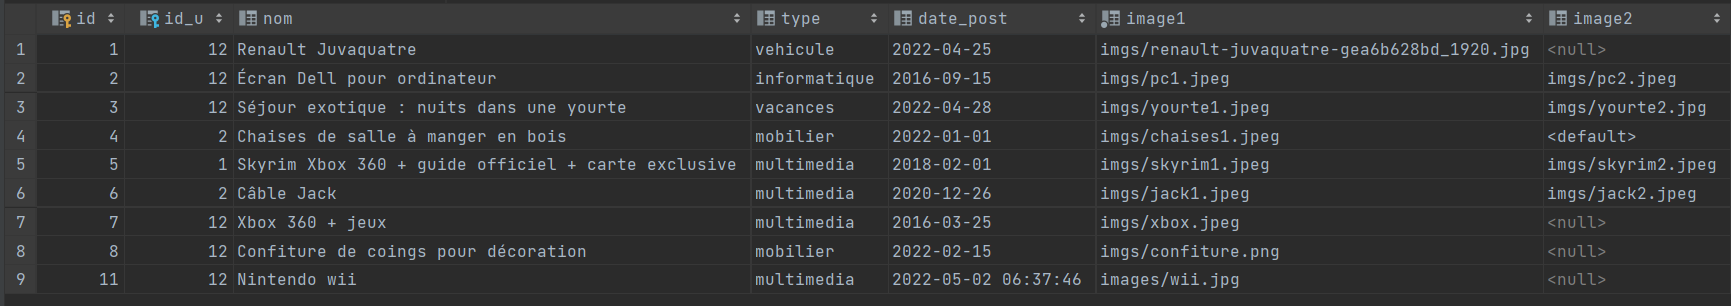
\includegraphics[scale=0.45]{annonce_p1.PNG}
        \caption{Exemple de données présentent dans la table \emph{annonce\_p} partie 1}
        \label{fig1}
    \end{figure}

    \begin{figure}[ht]
        \centering
        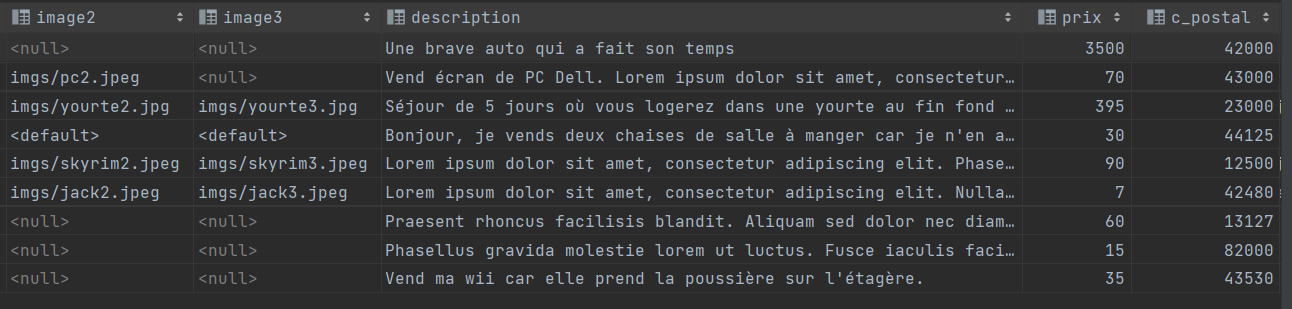
\includegraphics[scale=0.5]{annonce_p2.PNG}
        \caption{Exemple de données présentent dans la table \emph{annonce\_p} partie 1}
        \label{fig2}
    \end{figure}

    \item La table \emph{user}, il s'agit de la table liée aux utilisateurs du site.\\
    Les utilisateurs sont définis par :
    \begin{itemize}
        \item \textbf{un identifiant} unique à chaque utilisateur
        \item \textbf{un genre} 
        \item \textbf{un prénom}
        \item \textbf{un nom}
        \item \textbf{une date de naissance}
        \item \textbf{un pseudo}
        \item \textbf{un mot de passe} crypté en MD5 (Message Digest 5)
        \item \textbf{un email} afin de pouvoir envoyer un email
        \item \textbf{un statut} afin de savoir si l'utilisateur est un administrateur ou pas.
    \end{itemize}
\end{enumerate}

\begin{figure}[ht]
    \centering
    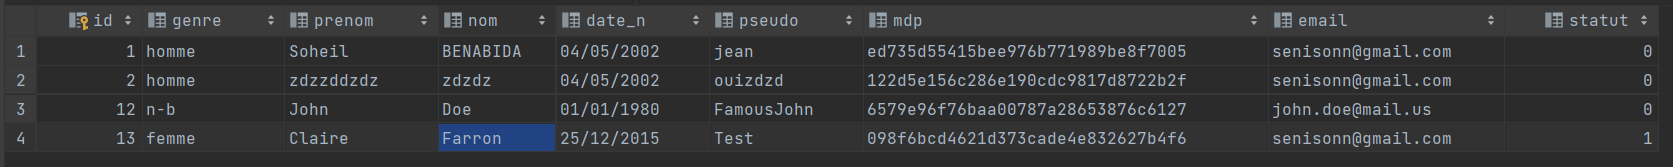
\includegraphics[scale=0.5]{user.PNG}
    \caption{Exemple de données présentent dans la table \emph{user}}
    \label{fig3}
\end{figure}

\section{Le déroulement du projet}
Contrairement à ce que nous aurions pu penser, le projet ne s'est pas dérouler sans encombre. Nous avons tous rencontré au moins une difficultée durant toute la durée du projet.\\
Pour Lina, son problème était lié a l'insertion d'images dans la base de données afin de régler ce problème elle a repris son code de A à Z.\\
Pour Mathis, il a rencontré un problème lors de la mise en page en CSS après avoir réaliser que l'utilisation de Boostrap ne serait pas comptabilisé. Il a donc décider de remplacer boostrap par du CSS pur et d'utiliser des flexbox.\\
Il a également rentré un problème lors de l'implémentation de la ``Sticky navbar''.\\
Enfin Soheil a eu un problème indépendant de sa volonté, en effet, un paquet PHP de son ordinateur s'était désinstallé.

\section{Quelques remarques}
\subsection*{Lina}
\subsection*{Soheil}
\subsection*{Mathis}
Pour les prochaines années, essayer de banaliser une semaine afin de permettre aux étudiants de se concentrer entièrement sur le projet. 
\end{document}
